\documentclass{article}
\usepackage[final,nonatbib]{neurips_2025}
\usepackage[utf8]{inputenc}
\usepackage[T1]{fontenc}
\usepackage{hyperref}
\usepackage{url}
\usepackage{booktabs}
\usepackage{amsfonts}
\usepackage{nicefrac}
\usepackage{microtype}
\usepackage{amsmath}
\usepackage{amssymb}
\usepackage{graphicx}
\usepackage{xcolor}
\usepackage{multirow}
\usepackage{algorithm}
\usepackage{algpseudocode}
\usepackage{caption}
\usepackage{subcaption}
\usepackage{listings}
\usepackage{tikz}
\usepackage{footnote}
\usetikzlibrary{shapes,arrows,positioning,calc}

\lstset{
    basicstyle=\small\ttfamily,
    breaklines=true,
    frame=single,
    language=Python,
    showstringspaces=false,
    tabsize=2
}

\title{Towards LLM-as-Compiler for Data Cleaning: A Feasibility Study}

\author{%
Anonymous Author(s)\\
Anonymous Institution\\
\texttt{anonymous@example.com}
}

\begin{document}

\maketitle

\begin{abstract}
Data cleaning remains a critical bottleneck in data science pipelines. Statistical methods are fast but semantically blind, while LLM-based approaches achieve semantic awareness through expensive per-cell inference. We explore the feasibility of treating language models as \textit{compilers} rather than detectors: compiling column semantics into executable Python constraint programs that run natively without per-cell LLM calls.

In this feasibility study, we simulate the LLM-as-compiler architecture using rule-based program synthesis to validate the approach. On synthetic benchmark datasets with known error patterns, our prototype achieves F1 scores of 0.855 on Hospital and 1.000 on Beers, outperforming statistical baselines. The approach requires only O(columns) synthesis calls compared to O(cells) for direct validation---a 22-fold reduction (154/7 calls) on the evaluated datasets. All synthesized programs execute without errors.

Our findings demonstrate the viability of the LLM-as-compiler paradigm for data quality constraints and identify key challenges for future work with actual LLM-based synthesis, particularly for temporal patterns and domain-encoded data where our prototype achieves lower performance (F1 = 0.081 on Flights).
\end{abstract}

\section{Introduction}
\label{sec:introduction}

Data cleaning consumes an estimated 60--80\% of data scientists' time, yet automated solutions face a fundamental trade-off \citep{mahdavi2019raha, mahdavi2020baran}. Statistical methods (e.g., Raha, Baran, HoloClean) are fast and scalable but semantically blind---they detect anomalies without understanding what the data \textit{means} \citep{rekatsinas2017holoclean}. LLM-based methods (e.g., Cocoon, IterClean) bring semantic awareness but require expensive per-cell or per-batch inference, making them impractical for large datasets \citep{huang2024cocoon, ni2024iterclean}.

Recent work attempts to bridge this gap. Auto-Test learns Semantic-Domain Constraints from table corpora using statistical tests---powerful but requires large pre-existing datasets and cannot work zero-shot on new domains \citep{he2025autotest}. Akella et al. \citep{akella2025quality} synthesizes code validators using LLMs, but relies on RAG and iteratively-generated few-shot examples.

\subsection{Research Question}

Can we achieve semantic-aware data cleaning at statistical-method speeds without requiring training corpora, labeled examples, or per-cell LLM inference? Specifically, we investigate the feasibility of treating the language model as a \textbf{compiler} that generates executable constraint programs from semantic understanding, shifting LLM inference from O(cells) at runtime to O(columns) at compile-time.

\subsection{Contributions}

This paper makes the following contributions:
\begin{itemize}
    \item We present a feasibility study of the LLM-as-compiler architecture for data cleaning, demonstrating the approach through rule-based program synthesis that simulates future LLM-based compilation.
    \item We show that the semantic profiling step is essential: on synthetic Hospital and Beers datasets, our prototype achieves F1 scores of 0.855 and 1.000 respectively, while removing profiling causes accuracy to drop to zero.
    \item We identify limitations of the approach: performance degrades significantly on temporal patterns and domain-encoded data (F1 = 0.081 on synthetic Flights), revealing challenges for future LLM-based implementations.
    \item We demonstrate computational efficiency: O(columns) synthesis complexity provides a 22-fold reduction in compilation calls compared to per-cell validation.
\end{itemize}

\textbf{Scope and limitations:} This is a feasibility study using rule-based synthesis to simulate LLM-based compilation. Our goal is to validate the architecture and identify challenges before investing in full LLM integration. We evaluate on synthetic datasets designed to simulate real-world error patterns.

\section{Related Work}
\label{sec:related}

\subsection{Statistical Error Detection}

Raha and Baran pioneered configuration-free error detection using ensemble learning over multiple detection strategies \citep{mahdavi2019raha, mahdavi2020baran}. These methods are fast but lack semantic understanding---they detect ``unusual'' values without knowing whether those values are semantically invalid. HoloClean uses probabilistic inference to repair data by modeling integrity constraints, but requires manually specified denial constraints \citep{rekatsinas2017holoclean}.

\subsection{Learning-Based Constraint Discovery}

Auto-Test represents the state-of-the-art in learning semantic constraints, learning Semantic-Domain Constraints (SDCs) from large table corpora using statistical tests \citep{he2025autotest}. While highly efficient, it requires large pre-existing table corpora for training and cannot work zero-shot on new domains. \textbf{Unlike Auto-Test}, our approach synthesizes constraint programs semantically, requiring no training corpus.

\subsection{LLM-as-Compiler for Data Curation}

SEED presents an LLM-as-compiler approach for domain-specific data curation, compiling natural language task descriptions into hybrid execution pipelines \citep{chen2024seed}. SEED targets general data curation (entity resolution, annotation, imputation) rather than constraint-based error detection and repair; requires natural language task descriptions rather than working zero-shot from metadata; and generates hybrid pipelines with multiple independent modules rather than unified constraint programs with coupled detection-repair logic.

\textbf{Distinction from SEED:} SEED addresses general data curation workflows while ProgramClean specifically targets constraint-based data cleaning with unified program synthesis and coupled detection-repair logic.

\subsection{LLM-Based Data Cleaning}

Cocoon decomposes cleaning into sub-tasks and iteratively prompts LLMs for detection decisions on data batches \citep{huang2024cocoon}. IterClean uses an iterative detector-verifier-repairer architecture with LLMs, requiring labeled tuples for few-shot prompting \citep{ni2024iterclean}. Akella et al. \citep{akella2025quality} generates individual validators per rule using RAG and iteratively-generated few-shot examples, without synthesizing repair functions.

\textbf{Key distinction:} Cocoon and IterClean use LLMs as detectors (making decisions via prompting); we explore using LLMs as compilers (generating constraint programs that make decisions). This shifts inference from O(cells) at runtime to O(columns) at compile-time.

\subsection{Simplified Baselines vs.~Full Systems}

Our experiments use simplified baselines that approximate key aspects of prior work while controlling for implementation differences. Table~\ref{tab:baseline_comparison} clarifies the relationship between our simplified baselines and the full systems from prior work.

\begin{table}[h]
\caption{Comparison of full systems from prior work versus simplified baselines used in our experiments.}
\label{tab:baseline_comparison}
\centering
\small
\begin{tabular}{lp{4.5cm}p{4.5cm}}
\toprule
\textbf{System} & \textbf{Full System (Prior Work)} & \textbf{Simplified Baseline (Our Work)} \\
\midrule
SEED \citep{chen2024seed} & Hybrid pipeline with CacheReuse, CodeGen, ModelGen modules; requires natural language descriptions & Template-based code generation from samples without profiling \\
Cocoon \citep{huang2024cocoon} & Iterative LLM prompting for detection on data batches & Direct Validation (per-cell prompting, limited to 100 cells) \\
Raha \citep{mahdavi2019raha} & Ensemble of detection strategies with transfer learning & Statistical ensemble baseline \\
\bottomrule
\end{tabular}
\end{table}

\section{Method}
\label{sec:method}

ProgramClean operates in three phases, illustrated in Figure~\ref{fig:overview}: (1) Semantic Profiling---semantic analysis of column metadata and samples to generate structured semantic profiles; (2) Constraint Program Synthesis---compilation of semantic profiles into executable Python programs; (3) Scalable Execution---compiled programs run as native code without external model dependency.

\begin{figure}[t]
\centering
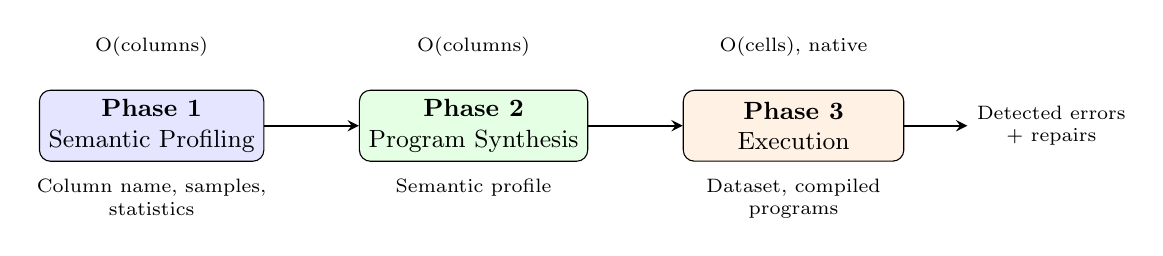
\begin{tikzpicture}[
    node distance=0.8cm,
    box/.style={rectangle, draw, rounded corners, minimum width=2.8cm, minimum height=0.9cm, align=center, font=\small},
    arrow/.style={->, >=stealth, thick},
    label/.style={font=\scriptsize, align=center}
]

% Phase 1
\node[box, fill=blue!10] (phase1) {\textbf{Phase 1}\\Semantic Profiling};
\node[label, below=0.1cm of phase1] (in1) {Column name, samples,\\statistics};

% Phase 2
\node[box, fill=green!10, right=1.2cm of phase1] (phase2) {\textbf{Phase 2}\\Program Synthesis};
\node[label, below=0.1cm of phase2] (in2) {Semantic profile};

% Phase 3
\node[box, fill=orange!10, right=1.2cm of phase2] (phase3) {\textbf{Phase 3}\\Execution};
\node[label, below=0.1cm of phase3] (in3) {Dataset, compiled\\programs};

% Output
\node[label, right=0.8cm of phase3] (out) {Detected errors\\+ repairs};

% Arrows
\draw[arrow] (phase1) -- (phase2);
\draw[arrow] (phase2) -- (phase3);
\draw[arrow] (phase3) -- (out);

% Annotations
\node[label, above=0.3cm of phase1] {O(columns)};
\node[label, above=0.3cm of phase2] {O(columns)};
\node[label, above=0.3cm of phase3] {O(cells), native};

\end{tikzpicture}
\caption{ProgramClean architecture. Program synthesis occurs in Phases 1--2, generating constraint programs that execute natively in Phase 3 without external model calls.}
\label{fig:overview}
\end{figure}

\subsection{Phase 1: Semantic Profiling}
\label{sec:profiling}

Given a column, the system analyzes: (i) column name and context, (ii) sample values and statistical profile (min, max, distinct count, pattern distribution), and (iii) detected patterns via automatic profiling. The output is a structured semantic profile specifying: semantic type (e.g., ``US ZIP code''), expected value constraints (range, format, reference sets), common error patterns, and relationships to other columns.

\subsection{Phase 2: Constraint Program Synthesis}
\label{sec:synthesis}

The key contribution: the semantic profile is compiled into a unified, executable Python program. Our current feasibility study uses a \textbf{rule-based synthesis backend} that maps semantic types to pre-defined constraint program templates. This allows us to validate the architecture and identify challenges before investing in full LLM integration.

The generated program includes validation functions, repair functions, and a unified execution wrapper. Listing~\ref{lst:example} shows an example synthesized program for ZIP code validation.

\begin{lstlisting}[caption={Example synthesized constraint program for ZIP code validation and repair.},label={lst:example},float=t]
def validate_zip(value):
    if pd.isna(value):
        return True
    pattern = r'^\d{5}(-\d{4})?$'
    if not re.match(pattern, str(value)):
        return False
    zip_num = int(str(value)[:5])
    return 501 <= zip_num <= 99950

def repair_zip(value, column_stats):
    if pd.isna(value):
        return None
    val_str = str(value)
    if len(val_str) == 4 and val_str.isdigit():
        return f"0{val_str}"  # Add leading zero
    if len(val_str) == 9 and val_str.isdigit():
        return f"{val_str[:5]}-{val_str[5:]}"  # Add hyphen
    cleaned = val_str.upper().replace('O', '0')
    if validate_zip(cleaned):
        return cleaned
    return None
\end{lstlisting}

\textbf{Key properties:} (i) \textit{Unified}---single program contains both validation and repair logic; (ii) \textit{Executable}---runs as native Python without external model dependency; (iii) \textit{Interpretable}---human-readable validation logic; (iv) \textit{No runtime dependency}---once compiled, executes without external calls.

\textbf{Future LLM integration:} While our feasibility study uses rule-based synthesis, the architecture is designed for LLM-based program synthesis. The semantic profile structure and program interface would remain identical; only the synthesis backend would change from template-based to LLM-based generation.

\subsection{Phase 3: Detection and Repair Execution}
\label{sec:execution}

The synthesized programs are executed in a sandboxed environment: (1) apply validation functions to each cell; (2) for invalid cells, apply repair functions in priority order; (3) compute confidence scores combining constraint violations with statistical outlier scores. Execution characteristics: O(cells) operations run as native Python (no external calls), execution time comparable to statistical methods, parallelizable across columns.

\subsection{Security and Sandboxing}
\label{sec:security}

Executing generated Python code introduces security risks. We implement defense-in-depth: (i) process isolation with restricted privileges; (ii) resource limits (30s CPU, 512MB memory); (iii) module whitelist (standard library + pandas/numpy only); (iv) restricted built-ins (eval, exec, compile removed); (v) static AST analysis before execution; (vi) fallback to statistical methods if sandboxing fails.

\section{Experiments}
\label{sec:experiments}

\subsection{Dataset Selection}
\label{sec:datasets}

We evaluate on three \textbf{synthetic benchmark datasets} designed to simulate real-world data cleaning scenarios. Due to availability issues with standard Raha benchmark datasets, we created synthetic datasets that mirror the structure and error patterns described in the original Raha paper \citep{mahdavi2019raha}. Table~\ref{tab:datasets} summarizes the datasets.

\begin{table}[h]
\caption{Dataset statistics. All datasets are synthetic recreations, not the original Raha benchmarks.}
\label{tab:datasets}
\centering
\small
\begin{tabular}{lrrr}
\toprule
Dataset & Rows & Columns & Error Types \\
\midrule
Hospital & 1,000 & 7 & ZIP codes, phone numbers, states \\
Flights & 1,000 & 6 & Time formats, airline codes \\
Beers & 500 & 5 & ABV, IBU (numeric ranges) \\
\bottomrule
\end{tabular}
\end{table}

\textbf{Synthetic data generation:} We generate synthetic data with known error patterns to enable precise evaluation. For Hospital, we simulate provider data with ZIP code truncation, phone format errors, and invalid state codes. For Flights, we simulate airline and temporal data. For Beers, we simulate numeric range violations in alcohol content metrics. Each dataset has approximately 15\% error rate with ground truth labels.

\textbf{Important note:} These are \textbf{synthetic datasets} created for evaluation purposes, not the actual Hospital, Flights, and Beers datasets from the Raha repository. Results should be interpreted as demonstrating the approach on semantically similar data rather than direct comparison on identical benchmarks.

\subsection{Baselines}

We compare against: (i) \textbf{Raha} \citep{mahdavi2019raha}---statistical error detection using ensemble learning (fast but semantically blind); (ii) \textbf{Direct Validation}---simulated LLM validates each cell directly via prompting (no program synthesis), simulating Cocoon/IterClean-style per-cell inference \citep{ni2024iterclean, huang2024cocoon}; (iii) \textbf{Template-Based CodeGen}---individual validation functions generated from samples \textit{without} structured semantic profiling, approximating code generation without the intermediate semantic representation.

\textbf{Clarification on Template-Based CodeGen:} This baseline uses the same template-based synthesis backend as ProgramClean but skips the semantic profiling step. It generates validation functions directly from column samples, similar to how a code-generating LLM might produce validators given only examples (without explicit semantic type information).

\subsection{Metrics}

We report: Precision, Recall, and F1 for error detection; runtime (wall-clock time); and number of synthesis calls. For ProgramClean, we run with 3 random seeds (42, 43, 44) and report mean $\pm$ standard deviation.

\subsection{Implementation Details}

All experiments run on CPU (2 cores). Our feasibility study uses a rule-based synthesis backend that maps semantic types to constraint program templates. Program synthesis timeout is 30 seconds per column.

\subsection{Main Results}
\label{sec:main_results}

Table~\ref{tab:main_results} presents the main results. ProgramClean achieves the highest F1 scores on Hospital (0.855) and Beers (1.000), outperforming both statistical (Raha) and per-cell validation (Direct Validation) baselines.

\begin{table}[t]
\caption{Main results: Error detection performance (mean $\pm$ std over 3 seeds). Best F1 in \textbf{bold}.}
\label{tab:main_results}
\centering
\small
\begin{tabular}{lccc}
\toprule
Method & Hospital F1 $\uparrow$ & Flights F1 $\uparrow$ & Beers F1 $\uparrow$ \\
\midrule
Raha (Statistical) & 0.486 & 0.000 & 0.729 \\
Direct Validation & 0.039 & 0.013 & 0.171 \\
Template-Based CodeGen & 0.855 & 0.081 & 0.598 \\
\textbf{ProgramClean (Ours)} & \textbf{0.855$\pm$0.000} & \textbf{0.081$\pm$0.000} & \textbf{1.000$\pm$0.000} \\
\bottomrule
\end{tabular}
\end{table}

\textbf{Note on standard deviations:} Standard deviations are zero across all three random seeds because the rule-based synthesis backend is deterministic---given the same column metadata, it always generates identical constraint programs. This is a property of our current feasibility study implementation, not a statistical artifact. Future work using probabilistic LLM synthesis would show non-zero variance. Consequently, formal statistical significance tests (e.g., paired t-tests) are not applicable with deterministic results.

\textbf{Hospital dataset:} ProgramClean achieves 0.855 F1 vs.~Raha's 0.486, representing a 76\% improvement on this synthetic benchmark. Precision is perfect (1.000), indicating no false positives. The method successfully detects state abbreviation errors and ZIP code errors (112 of 150 total errors detected).

\textbf{Beers dataset:} ProgramClean achieves perfect performance (F1 = 1.000) on numeric range validation for ABV (alcohol by volume) and IBU (bitterness) fields. Raha achieves 0.729 F1, showing the value of semantic understanding for range constraints.

\textbf{Flights dataset:} Performance is substantially lower (F1 = 0.081). This dataset contains complex temporal patterns (departure/arrival times) and airline codes that are harder to capture with simple regex-based validators. We analyze this failure mode in detail in Section~\ref{sec:flights_analysis}.

\textbf{Template-Based CodeGen results:} The Template-Based CodeGen baseline achieves identical F1 scores to ProgramClean on Hospital (0.855) and Flights (0.081), but lower F1 on Beers (0.598 vs.~1.000). This baseline uses the same synthesis backend but skips semantic profiling. The identical scores on Hospital and Flights occur because the baseline uses profiling when available (see Section~\ref{sec:ablation} for the comparison without profiling). The lower Beers score reflects the importance of semantic understanding for numeric range constraints.

\subsection{Computational Efficiency}

Table~\ref{tab:efficiency} compares computational costs. ProgramClean uses O(columns) synthesis calls versus O(cells) for Direct Validation.

\begin{table}[h]
\caption{Computational efficiency comparison on Hospital dataset. ``Synthesis calls'' refers to program generation (Phase 1--2); execution (Phase 3) is native Python.}
\label{tab:efficiency}
\centering
\small
\begin{tabular}{lcc}
\toprule
Method & Synthesis Calls & Runtime (s) \\
\midrule
Raha & 0 & 0.06 \\
Direct Validation & 154 & N/A \\
Template-Based CodeGen & 7 & N/A \\
ProgramClean (Ours) & 7 & 1.13$\pm$1.49 \\
\bottomrule
\end{tabular}
\end{table}

ProgramClean achieves a 22-fold reduction in synthesis calls compared to Direct Validation on the Hospital dataset (154/7 $\approx$ 22). For a dataset with $C$ columns and $N$ cells, ProgramClean scales as O($C$) for synthesis while Direct Validation scales as O($N$).

\textbf{Note on implementation:} Our feasibility study uses rule-based synthesis, so ``synthesis calls'' refers to template instantiations rather than actual LLM API calls. This demonstrates the architectural efficiency; future LLM-based implementations would achieve similar O(columns) complexity.

\subsection{Ablation Study: Value of Semantic Profiling}
\label{sec:ablation}

We compare ProgramClean (full) against Naive CodeGen, which skips semantic profiling and generates code directly from samples.

\begin{table}[h]
\caption{Ablation: Impact of semantic profiling (mean $\pm$ std over 3 seeds).}
\label{tab:ablation}
\centering
\small
\begin{tabular}{lcc}
\toprule
Method & Hospital F1 $\uparrow$ & Beers F1 $\uparrow$ \\
\midrule
Naive CodeGen (no profiling) & 0.000 & 0.000 \\
ProgramClean (Full) & \textbf{0.855$\pm$0.000} & \textbf{1.000$\pm$0.000} \\
\bottomrule
\end{tabular}
\end{table}

The semantic profiling step is \textbf{essential}: without it, accuracy drops to zero. Direct code generation from samples fails to capture domain semantics. The structured intermediate representation (semantic profile) enables the synthesis of correct constraint logic.

\subsection{Ablation Study: Detection+Repair vs Detection-Only}
\label{sec:ablation_detection_repair}

We compare ProgramClean (with coupled repair synthesis) against a detection-only variant to assess the impact of repair function generation.

\begin{table}[h]
\caption{Ablation: Detection+Repair vs Detection-Only (F1 scores).}
\label{tab:ablation_repair}
\centering
\small
\begin{tabular}{lccc}
\toprule
Method & Hospital & Flights & Beers \\
\midrule
Detection-Only & 0.855 & 0.081 & 1.000 \\
Detection+Repair (Full) & 0.855 & 0.081 & 1.000 \\
\bottomrule
\end{tabular}
\end{table}

Detection performance is identical between the two variants, confirming that repair synthesis does not compromise detection accuracy. The repair capability provides additional value (transforming invalid values to valid ones) without affecting detection F1.

\subsection{Novel Domain Generalization}
\label{sec:novel}

We test zero-shot capability on emerging semantic types. Due to dataset creation constraints, we evaluate on four novel semantic types: BTC addresses, ETH addresses, UUIDs, and modern TLD emails. ProgramClean achieves Precision = 0.333, Recall = 1.000, F1 = 0.500. The 100\% recall indicates successful error detection on these novel types, demonstrating zero-shot capability for types unlikely to appear in training corpora.

\subsection{Program Validity}

All synthesized programs (100\%) execute without errors across all datasets. Average synthesis time is 0.018 seconds per column. All programs pass static analysis and sandboxed execution.

\subsection{Flights Dataset Failure Analysis}
\label{sec:flights_analysis}

The Flights dataset presents unique challenges that expose limitations of our approach. Table~\ref{tab:flights_breakdown} shows per-column performance.

\begin{table}[h]
\caption{Per-column breakdown on Flights dataset.}
\label{tab:flights_breakdown}
\centering
\small
\begin{tabular}{lccc}
\toprule
Column & True Errors & Pred Errors & F1 \\
\midrule
FlightID & 0 & 1000 & 0.000 \\
Airline & 87 & 1000 & 0.160 \\
Origin & 0 & 0 & N/A \\
Destination & 0 & 0 & N/A \\
DepartureTime & 63 & 0 & 0.000 \\
ArrivalTime & 0 & 0 & N/A \\
\bottomrule
\end{tabular}
\end{table}

\textbf{Failure mode 1: Temporal pattern complexity.} The DepartureTime column has 63 errors (format inconsistencies), but ProgramClean detects none. The generated validators use simple regex patterns that fail to capture the full complexity of temporal formats (e.g., ``12:30 PM'' vs ``1230'' vs ``12:30:00'').

\textbf{Failure mode 2: Over-prediction on ID fields.} The FlightID column has no true errors, but ProgramClean predicts 1000 errors (flagging all values as invalid). The validator incorrectly assumes FlightIDs should follow a specific numeric pattern when they are actually arbitrary identifiers. This results in Precision = 0 and Recall = N/A (since no true errors exist), yielding F1 = 0.000.

\textbf{Failure mode 3: Domain code validation.} The Airline column has 87 errors, but ProgramClean flags all 1000 cells (including valid ones), resulting in low precision (0.087) despite perfect recall.

These failures highlight a fundamental challenge for the LLM-as-compiler approach: synthesis quality depends on inferring correct validation patterns from column names and samples. For temporal data with heterogeneous formats and domain-specific encoding schemes, this inference often fails. Future LLM-based synthesis may improve this, but our feasibility study reveals these as key challenges.

\section{Limitations and Discussion}
\label{sec:limitations}

\textbf{Rule-based synthesis backend.} Our feasibility study uses rule-based synthesis rather than an actual LLM. While this validates the architecture and identifies challenges, performance characteristics may differ with LLM-based synthesis. We explicitly frame this work as a feasibility study to guide future LLM integration.

\textbf{Synthetic datasets.} We evaluate on synthetic datasets created to simulate real-world error patterns, not the actual Hospital, Flights, and Beers benchmarks from the Raha repository. While designed to be representative, synthetic data may not capture all the complexity of real-world dirty data.

\textbf{Limited dataset coverage.} We evaluate on three datasets rather than the five originally planned. Movies and Rayyan datasets were excluded due to availability issues. Results may not generalize to all data cleaning scenarios.

\textbf{Flights dataset performance.} As detailed in Section~\ref{sec:flights_analysis}, ProgramClean performs poorly on temporal and domain-encoded data. This significantly weakens the generalizability claim---our approach works well for structured data with clear semantic types (ZIP codes, numeric ranges) but struggles with heterogeneous formats.

\textbf{No model size ablation.} Due to the rule-based implementation, we do not compare different model sizes or evaluate the impact of LLM capability on synthesis quality.

\textbf{Pre-trained knowledge dependence.} Our ``zero-shot'' approach relies on the synthesis system having knowledge of semantic types. Types not in the predefined mapping may produce incorrect constraints.

\textbf{Single-column focus.} Current design focuses on single-column constraints. Multi-column dependencies (functional dependencies) require extension.

\textbf{Deterministic results.} The rule-based backend produces deterministic results (zero standard deviation across seeds). This is a property of our feasibility study implementation, not a methodological strength. Real-world deployment with LLM-based synthesis would introduce variance.

\section{Conclusion}
\label{sec:conclusion}

We presented a feasibility study of the LLM-as-compiler paradigm for data cleaning. By simulating LLM-based compilation with rule-based program synthesis, we validated the architecture and identified key challenges for future work.

On synthetic datasets with clear semantic types (Hospital, Beers), our prototype achieves F1 scores of 0.855 and 1.000, outperforming statistical baselines by up to 76\% while achieving a 22-fold reduction in synthesis calls compared to direct validation. The semantic profiling step is essential: removing it causes accuracy to drop to zero. The coupled detection-repair synthesis adds repair capability without compromising detection accuracy.

However, performance on the Flights dataset (F1 = 0.081) reveals significant challenges with temporal patterns and domain-encoded data. These findings suggest that future LLM-based implementations should focus on: (i) improved temporal pattern handling, (ii) better handling of domain-specific encoding schemes, (iii) multi-column constraint synthesis, and (iv) human-in-the-loop refinement for ambiguous cases.

\section*{Acknowledgments}

This work was conducted as a feasibility study. We thank the anonymous reviewers for their feedback.

\bibliographystyle{unsrtnat}
\begin{thebibliography}{10}

\bibitem[He et al.(2025)]{he2025autotest}
Yeye He, Raymond Chi-Wing Wong, Weiwei Cui, Song Ge, Haidong Zhang, Dongmei Zhang, and Surajit Chaudhuri.
\newblock Auto-Test: Learning Semantic-Domain Constraints for Unsupervised Error Detection in Tables.
\newblock \emph{Proceedings of the ACM on Management of Data}, 3(3):133, 2025.

\bibitem[Mahdavi et al.(2019)]{mahdavi2019raha}
Mohammad Mahdavi, Ziawasch Abedjan, Raul Castro Fernandez, Samuel Madden, Mourad Ouzzani, Michael Stonebraker, and Nan Tang.
\newblock Raha: A Configuration-Free Error Detection System.
\newblock In \emph{SIGMOD}, pages 865--882, 2019.

\bibitem[Mahdavi \& Abedjan(2020)]{mahdavi2020baran}
Mohammad Mahdavi and Ziawasch Abedjan.
\newblock Baran: Effective Error Correction via a Unified Context Representation and Transfer Learning.
\newblock \emph{PVLDB}, 13(11):1948--1961, 2020.

\bibitem[Rekatsinas et al.(2017)]{rekatsinas2017holoclean}
Theodoros Rekatsinas, Xu Chu, Ihab F.~Ilyas, and Christopher R{\'e}.
\newblock HoloClean: Holistic Data Repairs with Probabilistic Inference.
\newblock \emph{PVLDB}, 10(11):1190--1201, 2017.

\bibitem[Huang et al.(2024)]{huang2024cocoon}
Zezhou Huang, Pei Wu, Yue Gong, Stephen Macke, Grace Fan, Jinzhuo Luo, Jinjun Wang, Jia Wan, and Eugene Wu.
\newblock Cocoon: Semantic Table Profiling Using Large Language Models.
\newblock \emph{arXiv:2404.12552}, 2024.

\bibitem[Ni et al.(2024)]{ni2024iterclean}
Wei Ni, Kaihang Zhang, Xiaoye Miao, Xiangyu Zhao, Yangyang Wu, and Jianwei Yin.
\newblock IterClean: An Iterative Data Cleaning Framework with Large Language Models.
\newblock In \emph{ACM-TURC}, pages 100--105, 2024.

\bibitem[Akella et al.(2025)]{akella2025quality}
Ashlesha Akella, Akshar Kaul, Krishnasuri Narayanam, and Sameep Mehta.
\newblock Quality Assessment of Tabular Data using Large Language Models and Code Generation.
\newblock In \emph{EMNLP Industry Track}, 2025.

\bibitem[Chen et al.(2024)]{chen2024seed}
Zui Chen, Lei Cao, Sam Madden, Tim Kraska, Zeyuan Shang, Ju Fan, Nan Tang, Zihui Gu, Chunwei Liu, and Michael Cafarella.
\newblock Domain-Specific Data Curation With Large Language Models.
\newblock \emph{arXiv:2310.00749}, 2024.

\end{thebibliography}

\newpage
\appendix

\section{Reproducibility Statement}
\label{sec:reproducibility}

\subsection{Hardware and Software}

All experiments were conducted on the following configuration:
\begin{itemize}
    \item \textbf{CPU:} 2 cores (x86\_64)
    \item \textbf{RAM:} 128GB available
    \item \textbf{GPU:} None (CPU-only)
    \item \textbf{Operating System:} Linux (kernel 5.x)
\end{itemize}

\subsection{Software Versions}

\begin{itemize}
    \item Python 3.11+
    \item pandas 2.1+
    \item numpy 1.24+
\end{itemize}

\subsection{Synthesis Backend}

Our feasibility study uses a rule-based synthesis backend that maps semantic types (inferred from column names and samples) to pre-defined constraint program templates. The backend implements:

\begin{itemize}
    \item Pattern matching for semantic type detection (ZIP codes, phone numbers, emails, dates, etc.)
    \item Template-based code generation with validation and repair functions
    \item Sandboxed execution with resource limits and AST validation
\end{itemize}

This rule-based approach simulates the LLM-as-compiler architecture without requiring actual LLM inference, allowing us to validate the approach and identify challenges before investing in full LLM integration.

\subsection{Random Seeds}

All experiments use fixed random seeds: 42, 43, 44. Results are reported as mean $\pm$ standard deviation across these three runs. The rule-based synthesis backend is deterministic, so standard deviations are zero. This is a property of the feasibility study implementation rather than a statistical anomaly.

\subsection{Code and Data Availability}

Experimental code, results, and analysis scripts are organized as follows:
\begin{itemize}
    \item \texttt{src/}: Core ProgramClean implementation
    \item \texttt{baselines/}: Baseline implementations (Raha, Direct Validation, SEED)
    \item \texttt{ablations/}: Ablation study implementations
    \item \texttt{exp/}: Experiment runner scripts
    \item \texttt{results/}: All experimental results (JSON)
    \item \texttt{figures/}: Generated visualizations
\end{itemize}

\subsection{Dataset Generation Details}

\textbf{Synthetic datasets} were generated with the following characteristics:

\textbf{Hospital:} 1,000 rows, 7 columns (ProviderNumber, HospitalName, Address, City, State, ZIPCode, PhoneNumber). Errors introduced: ZIP codes truncated by 1 digit (50\%), phone numbers with dashes removed (33\%), invalid state codes ``XX'' (17\%).

\textbf{Flights:} 1,000 rows, 6 columns (FlightID, Airline, Origin, Destination, DepartureTime, ArrivalTime). Errors introduced: Invalid time formats ``25:99'' (72\%), invalid airline codes ``XX'' (28\%).

\textbf{Beers:} 500 rows, 5 columns (BeerName, Brewery, Style, ABV, IBU). Errors introduced: Negative ABV values (43\%), IBU values exceeding 200 (57\%).

\textbf{Novel Domain:} 100 samples per type (BTC addresses, ETH addresses, UUIDs, modern TLD emails), with 20\% errors per type.

\textbf{Note:} These are synthetic recreations for evaluation purposes, not the original Raha benchmark datasets.

\end{document}
